% Source: AESP_466_ClassWork/Supplements/Notes/latex/6.2.3/6.2.3.tex

\documentclass[border=4pt]{standalone}
\usepackage{amsmath,amssymb,amsthm}
\usepackage{graphicx}
\usepackage{tikz}
\usepackage{xcolor}
\usetikzlibrary{arrows.meta,calc,positioning,decorations.markings,patterns,shapes.geometric,angles,quotes}

\definecolor{Garnet}{HTML}{73000A}
\definecolor{USC_Rose}{HTML}{CC2E40}
\definecolor{USC_Blue}{HTML}{466A9F}
\definecolor{USC_Slate}{HTML}{1F414D}
\definecolor{USC_Olive}{HTML}{65780B}
\definecolor{USC_Lime}{HTML}{CED318}
\definecolor{USC_Gold}{HTML}{A49137}
\definecolor{USC_Black90}{HTML}{565556}
\definecolor{USC_Black10}{HTML}{ECECEC}

\newcommand{\vect}[1]{\mathbf{#1}}
\newcommand{\mat}[1]{\mathbf{#1}}
\newcommand{\uvec}[1]{\hat{\mathbf{#1}}}
\newcommand{\transpose}{^{\mkern-1.5mu\mathsf{T}}}
\newcommand{\inv}{^{-1}}
\newcommand{\deriv}[2]{\frac{d #1}{d #2}}
\newcommand{\pderiv}[2]{\frac{\partial #1}{\partial #2}}

\begin{document}
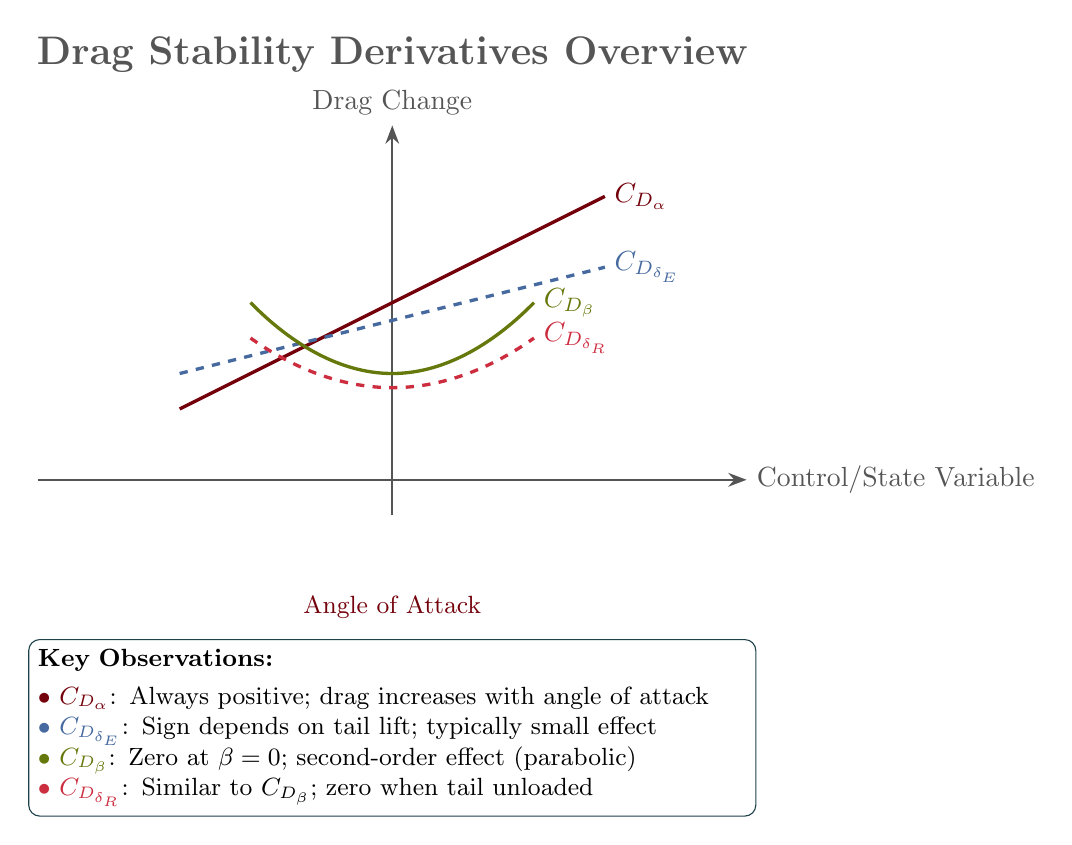
\begin{tikzpicture}[>=Stealth, scale=0.9]
    % Title
    \node[font=\Large\bfseries, USC_Black90] at (0,6) {Drag Stability Derivatives Overview};

    % Horizontal axis - control/state
    \draw[->, thick, USC_Black90] (-5,0) -- (5,0) node[right] {Control/State Variable};

    % Vertical axis - drag contribution
    \draw[->, thick, USC_Black90] (0,-0.5) -- (0,5) node[above] {Drag Change};

    % Alpha contribution (largest, positive slope)
    \draw[very thick, Garnet] (-3,1) -- (3,4);
    \node[Garnet, right] at (3,4) {$C_{D_\alpha}$};
    \node[Garnet, below, font=\small] at (0,-1.5) {Angle of Attack};

    % Elevator contribution
    \draw[very thick, USC_Blue, dashed] (-3,1.5) -- (3,3);
    \node[USC_Blue, right] at (3,3) {$C_{D_{\delta_E}}$};

    % Beta contribution (quadratic behavior near origin)
    \draw[very thick, USC_Olive] (-2,2.5) parabola bend (0,1.5) (2,2.5);
    \node[USC_Olive, right] at (2,2.5) {$C_{D_\beta}$};

    % Rudder contribution
    \draw[very thick, USC_Rose, dashed] (-2,2) parabola bend (0,1.3) (2,2);
    \node[USC_Rose, right] at (2,2) {$C_{D_{\delta_R}}$};

    % Annotation
    \node[draw=USC_Slate, fill=white, rounded corners, align=left, font=\small, text width=9cm] at (0,-3.5) {
        \textbf{Key Observations:}\\[0.3em]
        \textcolor{Garnet}{$\bullet$ $C_{D_\alpha}$}: Always positive; drag increases with angle of attack\\
        \textcolor{USC_Blue}{$\bullet$ $C_{D_{\delta_E}}$}: Sign depends on tail lift; typically small effect\\
        \textcolor{USC_Olive}{$\bullet$ $C_{D_\beta}$}: Zero at $\beta=0$; second-order effect (parabolic)\\
        \textcolor{USC_Rose}{$\bullet$ $C_{D_{\delta_R}}$}: Similar to $C_{D_\beta}$; zero when tail unloaded
    };

\end{tikzpicture}
\end{document}
